
%!TEX encoding = UTF-8 Unicode
\documentclass{simpleslides}

\author{Björn Regnell \\ \vspace{1em}{\small \url{https://cs.lth.se/bjorn-regnell}}}
\title{Introduction to Software\\Requirements Engineering}

\date{\footnotesize Version: \today}
\begin{document}
\maketitle

%AI images generated from https://perchance.org/ai-text-to-image-generator

% \begin{frame}[fragile]{About Björn Regnell}
% \begin{minipage}[t][1.0\textheight]{0.78\textwidth}
% \vspace{0pt}
% \begin{itemize}
% \item Professor in Software Engineering at the Faculty of Engineering, LTH, Lund University, Sweden.
% \item Research areas: 
% \begin{itemize}
% \item Software Engineering
% \item Requirements Engineering 
% \item Empirical research methods in Software Engineering 
% \end{itemize}
% \item Current teaching: 
% \begin{itemize}
% \item Software Requirements Engineering
% \item Introduction to Programming in Scala 
% \end{itemize}
% \item Homepage: 
% \begin{itemize}
% \item \url{https://cs.lth.se/bjorn-regnell}
% \end{itemize}
% \end{itemize}
% \end{minipage}%
% \hspace*{1em}\begin{minipage}[t][1.0\textheight]{0.22\textwidth}
% \vspace{0pt}\hfill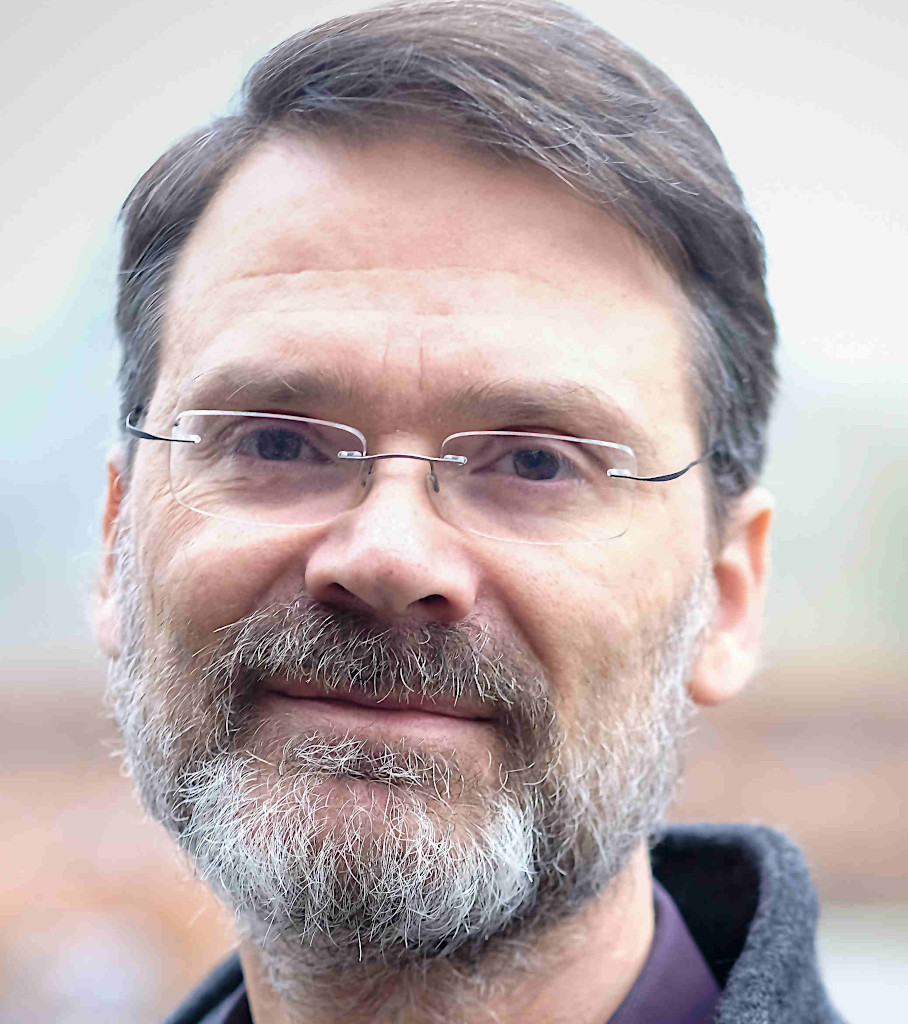
\includegraphics[width=0.9\textwidth]{img/bjorn-regnell}
% \end{minipage}%
% \end{frame}

\begin{frame}[fragile]{What is Requirements Engineering (RE)?}
%\begin{minipage}[t]{0.6\textwidth}
%\vspace{0pt}
\begin{itemize}
\item  Requirements Engineering (RE) is a sub-discipline of Software Engineering (SE) that is focused on the \textit{requirements} of software-intensive systems and their \textit{context}, which includes users and surrounding systems.
\item When you work with anything related to the \textit{decision-making process} of software development and its \emph{underlying intentions} you are doing requirements engineering.
\end{itemize}
%\end{minipage}%
\begin{minipage}[t]{0.4\textwidth}
\vspace{0pt}\hfill
\includegraphics[width=0.8\textwidth]{img/phone}
\end{minipage}%
\hspace{2em}\begin{minipage}[t]{0.5\textwidth}
\vspace{1em} 
Building shared knowledge \\ Making decisions \\ Communicating intent \\ Creating the future
\end{minipage}%
  
\end{frame}

\begin{frame}[fragile]{What is a requirement?}
\begin{minipage}[t]{0.6\textwidth}
\vspace{0pt}
\begin{itemize}
\item Something needed or wanted.
\item A documented representation of \\something needed or wanted.
\item The word ''requirement'' can have different meanings:
\begin{itemize}
\item ... must, wish, idea, design detail, rationale, ...
\end{itemize}
\item The most general meaning:\\
\emph{any} kind of information entity used in RE
\item You don't always get what you want and you often want things that you don't need
\end{itemize}
\end{minipage}%
\begin{minipage}[t]{0.4\textwidth}
  \vspace{0pt}
  \hfill

\includegraphics[width=0.8\textwidth]{img/light-bulb3}
\end{minipage}%
\end{frame}

\begin{frame}[fragile]{Activities in Requirements Engineering}
The work you do withing Requirements Engineering is often described in terms of these four activities:
\begin{itemize}
\item \textbf{Elicitation}: learn, invent, agree
\item \textbf{Specification}: represent, persist, evolve, communicate
\item \textbf{Validation}: check if requirements models are good enough
\item \textbf{Selection}: prioritize, decide, plan
\end{itemize}
\vspace*{1em}
\begin{minipage}[t]{0.6\textwidth}
\vspace{0pt}
These activities are often conducted \textbf{concurrently} and \textbf{iteratively}.
\end{minipage}%
\begin{minipage}[t]{0.4\textwidth}
\vspace{0pt}
\hfill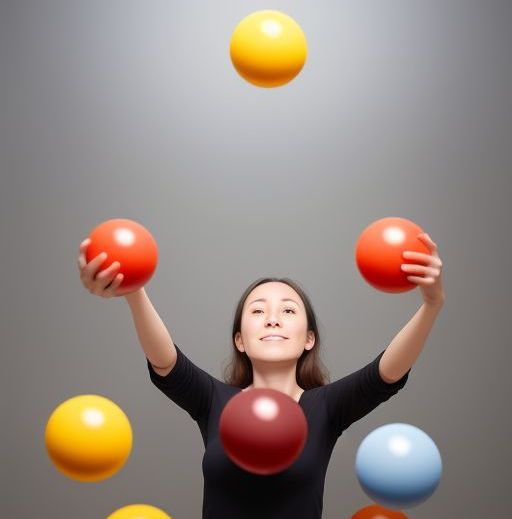
\includegraphics[width=0.8\textwidth]{img/juggling-cropped}
\end{minipage}%

\end{frame}

\begin{frame}[fragile]{The Context of Requirements Engineering}
%\begin{itemize}
%\item 
How to best do RE is \textbf{highly context-dependent}:
\begin{itemize} 
\item \textbf{Stakeholder configuration}: relation customer -- supplier
\\\textit{Type of Customer}: business partner, public authority, private consumer on a market
\\\textit{Type of Supplier}: consultancy, product integrator, subcontractor, open-source contributor in a community
\item \textbf{The funding model}, risk-sharing customer -- supplier:
\\not-for-profit/donation, internal use, share of sales, fixed license fee, service subscription, freemium, ad-based, ... 
\item \textbf{Level of customization}:
\\generic, customized, customer specific
\item \textbf{Hardware integration}:
\\pure software, hardware + software
\item \textbf{Network integration}:
\\stand-alone, connected, distributed
\item \textbf{Delivery model}:
\\one-off, eventually updated, continuous delivery
\end{itemize}
%\end{itemize}
\end{frame}

\begin{frame}[fragile]{Requirements Modelling}
\begin{minipage}[t]{0.6\textwidth}
\vspace{0pt}
\begin{itemize}
\item Finding the right representation:
\begin{itemize}
\item What is fit for purpose?
\item What is good enough?
\item When are we ''ready''?
\end{itemize}
\item Functionality and quality
\item Requirements at different levels
\item Living with incompleteness, ambiguity, inconsistency, ...
\end{itemize}
\end{minipage}%
\begin{minipage}[t]{0.4\textwidth}
\vspace{0pt}
\hfill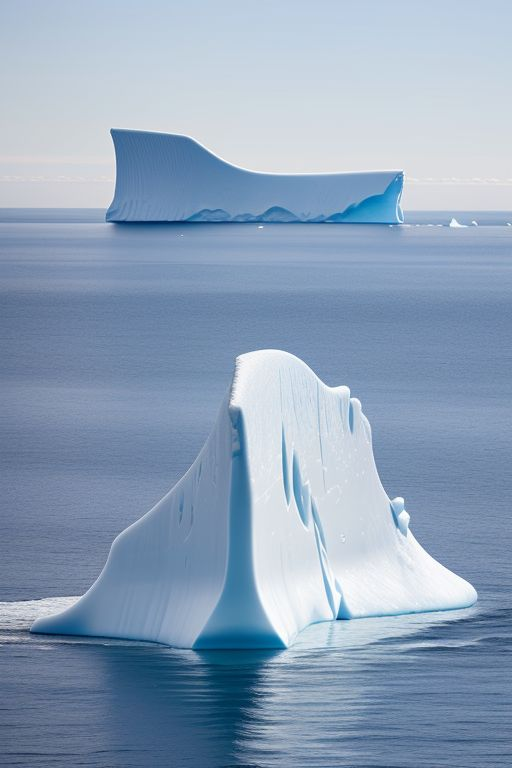
\includegraphics[width=0.8\textwidth]{img/iceberg4}
\end{minipage}%
\end{frame}

\begin{frame}[fragile]{Good enough requirements representations}
What is a good enough requirements model?
\\ \vspace*{0.5em}Examples of quality aspects, achievable to some degree:
\begin{itemize}
\item \textbf{Correctness}: reflect the expected, intended behavior
\item \textbf{Unambiguity}: stakholders have similar interpretation
\item \textbf{Completeness}: most important, relevant aspects included
\item \textbf{Consistency}: no contradictions among requirements
\item \textbf{Conciseness}: suitable level of abstraction and detail 
\item \textbf{Comprehensibility}: understood by stakeholders 
\item \textbf{Verifiability}: possible to check fulfillment 
\item \textbf{Feasibility}: possible to implement, value to justifiable cost 
\item \textbf{Traceability}: can be referred to, can find its origin
\item \textbf{Modifyability}: easy to change, good structure
\item \textbf{Ranked}: includes assessment of importance and stability
\end{itemize}
\end{frame}

\begin{frame}[fragile]{Requirements on System Functionality}
\begin{minipage}[t]{0.7\textwidth}
\vspace{0pt}
\begin{itemize}
\item \textbf{Data}: information stored by the system 
\begin{itemize}
\item domain-specific data entities
\item format of input and output data
\item representation of (externally visible) system state
\end{itemize}
\item \textbf{Logic}: computing input from output 
\begin{itemize}
\item logical behavior, state transitions
\item specifying desired output given:
\begin{itemize}
  \item expected and unexpected input
  \item current system state
  \item relevant usage situations
\end{itemize}
\item create, read, update, delete
\end{itemize}
\end{itemize}
\end{minipage}%
\begin{minipage}[t]{0.3\textwidth}
\vspace{0pt}
\hfill
\includegraphics[width=0.9\textwidth]{img/cogs}
\end{minipage}%
\end{frame}

\begin{frame}[fragile]{Requriements on System Quality}
\begin{itemize}
\item Goodness of implementation of intended functionality 
\begin{itemize}
  \item A level on a sliding scale.
  \item What is good enough?
  \item System-wide or specific to a certain feature?
\end{itemize}
\item Examples of quality aspects:
\begin{itemize}
\item \textbf{Accuracy}: Precisions of data.
\item \textbf{Capacity}: Resources per time unit.
\item \textbf{Performance}: Response time.
\item \textbf{Reliability}: Number of bugs, failure rate.
\item \textbf{Security}: Protect system from damage by malicious users. 
\item \textbf{Safety}: Protect users from being damaged by the system.
\item \textbf{Maintainability}: Easy to fix bugs and adapt the system.
\item \textbf{Usability}: Subjective and objective experience of users:\\ easy learn, supports my tasks, easy to remember, easy to understand, attractive: ''I like it!'' 
\end{itemize}
\end{itemize}
\end{frame}

\begin{frame}[fragile]{Requirements at Different Levels}
\begin{minipage}[t]{0.7\textwidth}
\vspace{0pt}
\begin{itemize}
\item Levels of Abstraction:\\the Goal-Design scale 
\item Levels of Detail: amount and richness of information 
\item Levels of Aggregation:\\grouping and linking 
\item Levels of Formality:\\from unstructured to mathematical
\begin{itemize}
\item Very informal: free-form representation, no explicit rules
\item Very formal: syntax, semantics, inference, meta-language
\item Formality enables automatic checks, concise models, ...
\item Formalization requires effort, knowledge, skills, ...
\end{itemize}
\end{itemize}
\end{minipage}%
\begin{minipage}[t]{0.35\textwidth}
\vspace{0pt}
\hfill
\includegraphics[width=0.9\textwidth]{img/stairs1}
\end{minipage}%
\end{frame}

\begin{frame}[fragile]{Levels of abstraction: The Goal-Design scale}
\begin{itemize}
\item Goal-level: represents the intentions of stakeholders; why? 
\item Domain-level: represents how users collaborate with the system to achieve their goals
\item Product-level: represents the relation between input and expected response; what?
\item Design-level:\\represents upfront decisions on system design, how?\\often based on existing systems and standards, often needs extra validation e.g. prototyping
\end{itemize}
\end{frame}

\begin{frame}[fragile]{Levels of Formality: a difficult tradeoff}

\begin{itemize}
\item Formality in various aspects to a varying degree: 
\begin{itemize}
  \item Very informal: free-form representation, no explicit rules\\examples: slide presentation, interview recording
  \item Very formal: all aspects of syntax, semantics, inference, meta-language are formalized\\example: state-machines, lambda calculus
\end{itemize}
\item Advantages of formalization:
\begin{itemize}
\item Reduced ambiguity
\item More concise models
\item Enables tooling: automatic checks, proof of soundness, ... 
\end{itemize}
\item Disadvantages of formalization:
\begin{itemize}
\item Harder to understand
\item Requires effort, specialized knowledge and skills
\item Limited in scope and expressive power
\item Some stakeholders cannot contribute in validation 
\end{itemize}
\end{itemize}
\end{frame}

\begin{frame}[fragile]{Automated support for RE}
Why tools?
\begin{itemize}
\item We want to boost our productivity.
\item The amount of information grows very quickly.
\item We need to adapt different views to specific stakeholders.
\item We need support for searching and summarizing.
\item Manual traceability management is very tedious!
\end{itemize}
Which tools?
\begin{itemize}
\item Generic tools for writing, drawing, databases, ...
\item Specialized tools, e.g. DOORS, Jira, openproject.org, ...
\item Artificial Intelligence for RE
\begin{itemize}
\item AI support to elicit, specify, validate, select 
\item Meta-level RE:\\RE for: AI for RE
\end{itemize}
\end{itemize}
\end{frame}

  

\begin{frame}[fragile]{Representing Feature Implementation Status}
Example state model of decision steps in feature refinement:
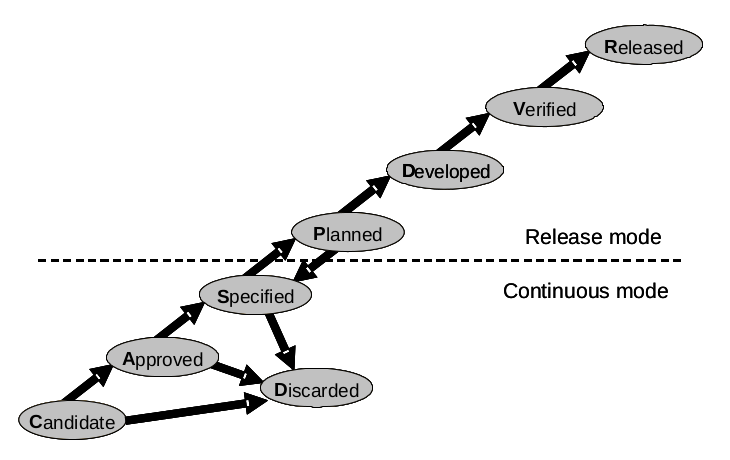
\includegraphics[width=0.9\textwidth]{img/ladder}
\\''The Feature Ladder''
\end{frame}

\begin{frame}[fragile]{Requirements Selection Quality}
\footnotesize
\textbf{If} we had perfect information about the all requirements \textbf{and} the ability to precisely predict the future \textbf{then} we could partition all requirements based on their quality (value versus cost) into:
\begin{itemize}\footnotesize
\item \textbf{Alfa}-requirements: should be \textit{selected} by perfect wisdom
\item \textbf{Beta}-requirements: should be \textit{rejected} by perfect wisdom
\end{itemize}
\begin{center}
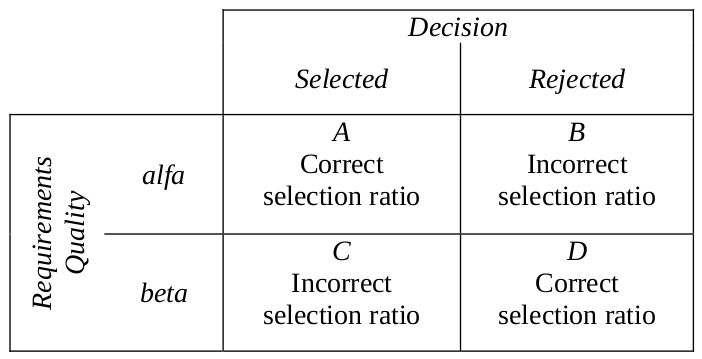
\includegraphics[width=0.7\textwidth]{img/alfa-beta-reqts}
\end{center}
{
Product quality: \hspace{0.5em}{\Large $\frac{A}{A + C}$}\hfill
Selection quality:\hspace{0.5em}{\Large $\frac{A + D}{A + B + C + D}$}
}
\end{frame}

\begin{frame}[fragile]{Requirements Prioritization: value versus cost}
Cost-value diagram with alfa- \& beta-requirements.
\begin{center}
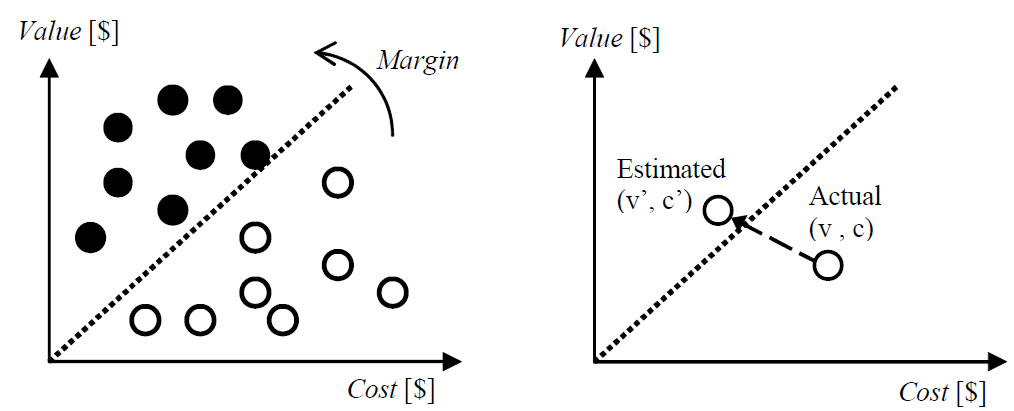
\includegraphics[width=1.0\textwidth]{img/cost-value}
\end{center}
Uncertain estimates of value \& cost $\rightarrow$ sub-optimal decisions.
\end{frame}

\begin{frame}[fragile]{Read until next time}

\begin{itemize}\footnotesize
%\item ''Requirements engineering challenges in market-driven software development -- An interview study with practitioners'' \\ L. Karlsson, Å. G. Dahlstedt, B. Regnell, J. Natt och Dag, A. Persson, \emph{Information and Software Technology} (2008) 
\item ''Market-Driven Requirements Engineering for Software Products'' \\ B. Regnell, S. Brinkkemper \\ \emph{Chapter 13 in the book ''Engineering and Managing Software Requirements'' Eds. Wholin \& Aurum},  ISBN 3 540 25043 3 (2005)
\end{itemize}

\end{frame}

\end{document}

